\documentclass[10pt,a4paper]{article}

\usepackage[utf8x]{inputenc}
\usepackage[norsk]{babel}
\usepackage[T1]{fontenc,url}
\usepackage[hang,small,bf]{caption}
\usepackage{relsize}
\usepackage{setspace}
\usepackage{parskip}
\usepackage{lmodern}
\usepackage{microtype}
\usepackage{verbatim}
\usepackage{amsmath, amssymb, amsthm}
\usepackage{mathtools}
\usepackage{tikz}
\usepackage{physics}
\usepackage{algorithm}
\usepackage{algpseudocode}
\usepackage{listings}
\usepackage{enumerate}
\usepackage{graphicx}
\usepackage{float}
\usepackage{hyperref}
\usepackage{varioref}
\usepackage{siunitx}
\usepackage{todonotes}
\usepackage{color}
\usepackage[margin=3cm]{geometry}
\labelformat{equation}{ligning~(#1)}

\renewcommand{\exp}{\mathrm{e}^}
\newcommand{\halflife}{t_{\frac{1}{2}}}
\newcommand{\half}{\frac{1}{2}}
\newcommand{\planck}{$h = \SI{6.626e-34}{J.s}$}

\definecolor{light_green}{rgb}{0, 0.6, 0}
\definecolor{light_grey}{rgb}{0.5, 0.5, 0.5}
\definecolor{magenta}{rgb}{0.7, 0, 0.5}


\lstdefinestyle{py}{
    language = python,
    frame = single,
    showstringspaces = false,
    basicstyle = \small\ttfamily,
    breaklines = true,
    commentstyle = \color{light_grey},
    keywordstyle = \color{magenta},
    stringstyle = \color{light_green},
}



\begin{document}
\section*{Oppgave 5.1 - Dra kasser}
\addcontentsline{toc}{section}{Oppgave 5.1 - Dra kasser - \texttt{pull\_blocks.py}}
Vi skal se på tilfellet der $N$ kasser som er festet sammen med et tau blir dratt av en person.
\begin{center}
	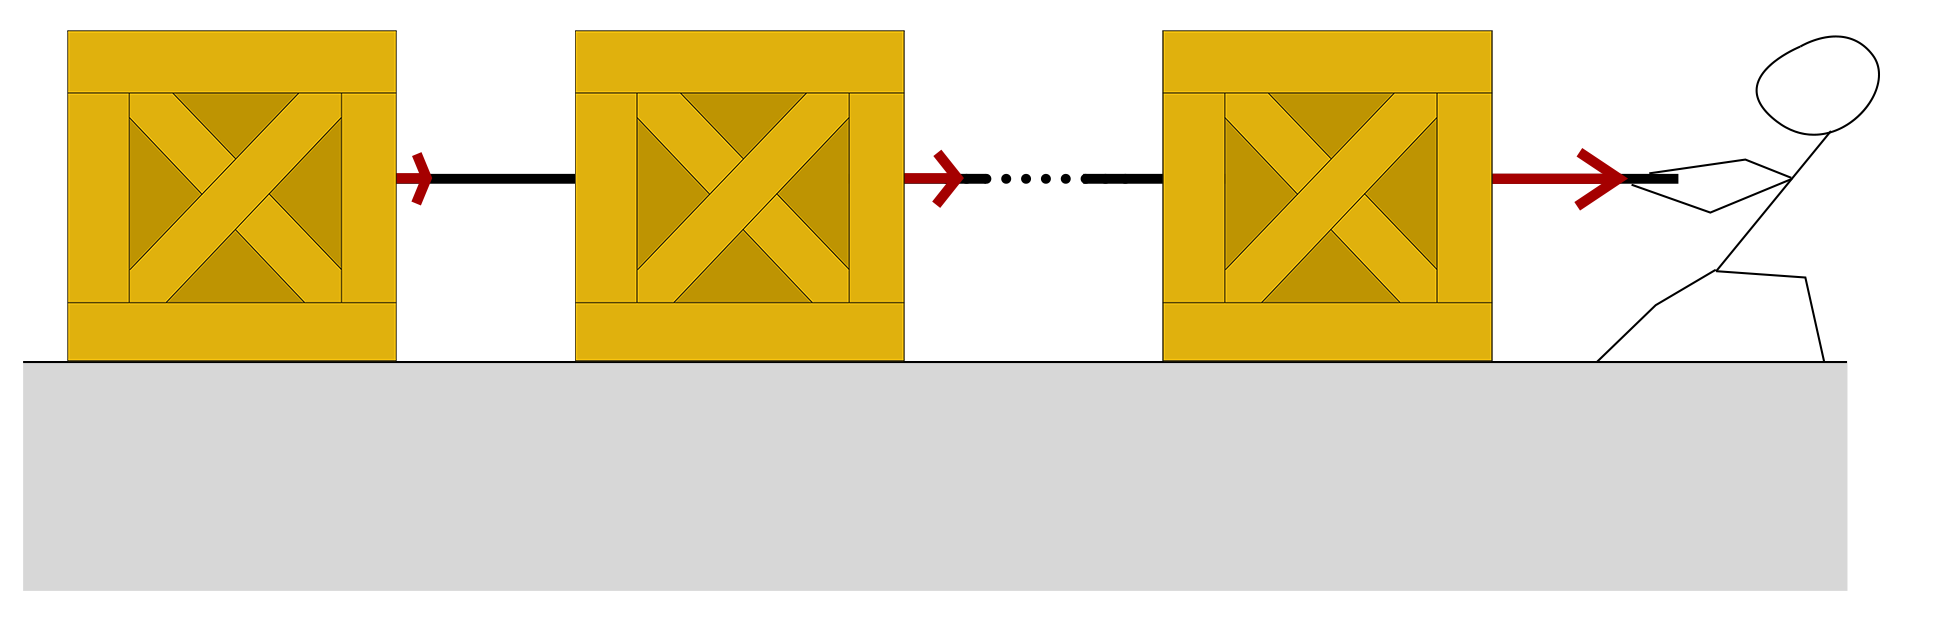
\includegraphics[scale=1]{fig_pull_crates-cp1.png}\\
	\captionof{figure}{Illustrasjon av en person som drar noen kasser.Prikkene mellom kassene indikerer at det er vilkårlig mange kasser. De røde pilene indikerer retninger og styrken på kreftene som virker på kassene.}
\end{center}

\subsection*{a)}
Vi har målt at hver $i$-te kasse blir påvirket av en kraft på $30 + 5\cdot i\,\si{\newton}$.
Lag et program som generer en liste av kreftene som virker på hver $i$-te kasse. Her har vi $N = 10$ kasser.

\subsection*{b)}
Det viser seg at de kreftene som ble målt i a), viste seg til å være for store. Del verdiene fra a) på 2 \textit{uten} å bruke for- eller while loops.
Summér så verdiene, også uten å bruke for- eller while loops, og skriv ut resultatet.

\textbf{Hint:} Her må vi bruke arrays.

Filnavn: \texttt{pull\_blocks.py}

\section*{Oppgave 5.2 - Plotting av relativistisk og klassisk bevegelsesmengde}
\addcontentsline{toc}{section}{Oppgave 5.2 - Plotting av relativistisk og klassisk bevegelsesmengde - \texttt{momentum\_plot.py}}
Bevegelsesmengden til et objekt med masse $m$ og hastighet $v$ er definert forskjellig i klassisk fysikk og i relativitetsteori.
\begin{align*}
p_{clas} &= m\cdot v
\\
p_{rel} &= m\cdot v\cdot \gamma, \ \ \ \ \gamma = \frac{1}{\sqrt{1-\frac{v^2}{c^2}}}
\end{align*}
Lyshastigheten er definert ved $c \approx 3\cdot 10^8\mathrm{m/s}$.

Sett $m = \SI{5}{kg}$ og plott funksjonene i samme plott med hastigheter jevnt fordelt i intervallet $v \in [0c,\ 0.9c] = [\SI{0}{m/s},\ \SI{2.7e8}{m/s}]$.

Filnavn: \texttt{momentum\_plot.py}



\section*{Oppgave 5.3 - Kondensatorutladning}
\addcontentsline{toc}{section}{Oppgave 5.3 - Kondensatorutladning - \texttt{capacitor\_vectorization.py}}
\textbf{Fysisk introduksjon:} En kondensator består av to metallplater satt opp parallelt mot hverandre. Hvis vi lader opp hver plate med henholdsvis positiv og negativ ladning (f.eks. ved å koble de til hver ende i et batteri), vil det dannes en spenning $V$ over kondensatoren. Hvis vi deretter kobler platene sammen med en ledning, vil strøm begynne å gå mellom platene, og kondensatoren vil utlades. For å hindre det i å gå uendelig mye strøm, setter vi på en motstand $R$ på ledningen mellom platene. Vi har nå en RC-krets.

Ladningen $Q$ til en kondensator som utlades i en RC krets er over tid gitt som
\begin{align*}
Q(t) = CV\exp{-t/RC}
\end{align*}
Følgende program regner ut denne utladningen for $n=1000$ tidssteg over et intervall $t = [\SI{0}{s},\ \SI{10}{s}]$. Kondensatoren har en kapasitans $C = \SI{0.007}{F}$, en initiell spenning $V_0 = \SI{50}{V}$, og kretsen har en motstand $R = \SI{350}{\Omega}$.
\lstinputlisting[style=py]{capacitor.py}
Kopier programmet og sjekk at det kommer opp et plott som synker i en bue.

Vektoriser programmet slik at \texttt{t\_list} og \texttt{I\_list} erstattes med numpy-arrays, og for loopene erstattes med vektor-operasjoner. Sjekk at resultatet fortsatt blir det samme.

Filnavn: \texttt{capacitor\_vectorization.py}




\section*{Oppgave 5.4 - Plancks Lov}
\addcontentsline{toc}{section}{Oppgave 5.4 - Plancks Lov - \texttt{Planck\_curves.py}}
Plancks lov beskriver hvor mye energi et svart legeme (som regel en stjerne) utstråler over et spekter av bølgelengder. Loven er gitt ved
\begin{align*}
B(\lambda) = \frac{2hc^2}{\lambda^5}\frac{1}{\exp{\frac{hc}{\lambda k T}}-1}
\end{align*}
der $T$ er temperaturen til stjernen, \planck\  er Planck's konstant, og $k = \SI{1.38e-23}{J/K}$ er Boltzmanns konstant. Lysets hastighet er fortsatt gitt som $c \approx \SI{3e8}{m/s}$. Kurvene som fremkommer av å plotte denne funksjonen over et spekter av bølgelengder kalles 'Planck-kurver', og de er et vanlig syn i fysikkbøker.


\subsection*{a)}
Sett temperaturen lik solens temperatur, $T = 5800\mathrm{K}$, og plott $B(\lambda)$ med bølgelengder jevnt fordelt i intervallet $\lambda \in [\SI{10}{nm},\ \SI{3000}{nm}] = [\SI{e-8}{m},\ \SI{3e-6}{m}]$


\subsection*{b)}
Inkluder også Planck-kurvene til stjernene Alpha Centauri A ($T=\SI{25000}{K}$) og Proxima Centauri ($T=\SI{2400}{K}$) i samme plott med Solen.

\subsection*{c)}
Wien's forskyvningslov forteller oss at toppunktet til Planck-kurvene skal ligge på bølgelengden
\begin{align*}
\lambda_{max} = \frac{b}{T}
\end{align*}
der $b = \SI{2.9e-3}{Km}$ kalles Wien's forskyvningskonstant.

Utvid plottet fra oppgave b) til å inkludere tre vertikal linjer ved $x = \lambda_{max}$ for hver av stjernene, og se at det stemmer med toppunktene til kurvene.

\textbf{Hint}: Du kan lage vertikale linjer med funksjonen \texttt{matplotlib.pyplot.axvline(x= )}

Filnavn: \texttt{Planck\_curves.py}



\section*{Oppgave 5.5 - Oscillerende fjær}
\addcontentsline{toc}{section}{Oppgave 5.5 - Oscillerende fjær - \texttt{oscilating\_spring.py}}
Hvis du henger en stein i enden av en fjær, trekker den ned en lengde $A$ og slipper, vil steinen oscillere opp og ned med en vertikal posisjon gitt etter formelen
\[	y(t) = A\cdot \exp{-\gamma t}\cos\left(\sqrt{\frac{k}{m}}\cdot t\right)
\]
Høyden $y=0$ korresponderer til posisjonen steinen vil ha når den henger løst i fjæren.\\
Steinen har en masse $m = \SI{9}{kg}$, og du trekker den ned en lengde $A = \SI{0.3}{m}$. Sett $k = \SI{4}{kg/s^2}$ og $\gamma = \SI{0.15}{s^{-1}}$.

\section*{a)}
Lag to tomme arrays \texttt{t\_array} og \texttt{y\_array} av lengde 101. Bruk en for loop til å fylle dem med tidsverdier i intervallet $[\SI{0}{s},\ \SI{25}{s}]$, og korresponderende $y(t)$ verdier.

\section*{b)}
Vektoriser koden ved bruk av numpy sin \texttt{linspace} funksjon, til å generere arrayet \texttt{t\_array}, og send den inn i en funksjon \texttt{y(t)} for å generere verdiene i \texttt{y\_array}. Programmet ditt skal på dette tidspunkt ikke inneholde noen loops.

\section*{c)}
Plott posisjonen til steinen mot tid i det gitte tidsintervallet. Bruk arrayene fra både deloppgave a) og b), og sjekk at grafene ligger helt oppå hverandre (sannsynligvis vil du ikke se den ene). Få korrekte enheter på begge akser.

Filnavn: \texttt{oscilating\_spring.py}





\section*{Oppgave 5.6 - Planetbaner}
\addcontentsline{toc}{section}{Oppgave 5.6 - Planetbaner - \texttt{planetary\_motion.py}}
Vi kan beskrive bevegelsen til en planet rundt en stjerne ved dens avstand til sin stjerne som en funksjon av hvor i banen planeten er:
\begin{equation}
r(\theta) = \frac{p}{1+e\cos(\theta)}	\label{eqn:radial_orbit}
\end{equation}
der $r$ er avstanden fra stjernen, og $\theta$ er hvilken vinkel i banen planeten har kommet til. $\theta = 0$ representerer vinkelen der planeten er nærmest stjernen.

$p$ er en parameter som sier noe om størrelsen på banen. Vi setter den til \SI{1}{AU}. \footnote{1 AU er den gjennomsnittlige avstanden mellom jorden og solen.}

$e$ kalles banens \textit{eksentrisitet}, og forteller oss hvor eliptisk banen er. $e = 0$ representerer en helt sirkulær bane, mens $e\geq 1$ beskriver en planet som ikke engang er i bane rundt stjernen, men bare passerer forbi.


\subsection*{a)}
Plott planetens distanse fra stjernen som en funksjon av dens angulære posisjon, $\theta$, for $e = 0$, $e=0.5$ og $e=0.8$ i samme plot. Bruk vinkler i intervallet $\theta \in [0,\ 2\pi]$, som altså tilsvarer én full bane rundt stjernen (vi regner i radianer). Få med korrekte enheter på begge akser.


\subsection*{b)}
Vi skal nå plotte den faktiske banen til planeten for hver av de tre eksentrisitetene. Vi dekomponerer \ref{eqn:radial_orbit} til $x$ og $y$ komponenter:
\[	x(\theta) = r(\theta)\sin(\theta),\ \ \ \ y(\theta) = r(\theta)\cos(\theta)
\]

Bruk disse ligningene til å plotte $y(\theta)$ mot $x(\theta)$ i det samme tidsintervallet, med de samme eksentrisitetene.

Husk at $r(\theta)$ og $\theta$ er arrays, slik at $x(\theta)$ og $y(\theta)$ blir også arrays uten videre, og kan plottes direkte mot hverandre.

\textbf{Hint:} Matplotlib holder ikke aksene proporsjonale i størrelse, slik at en sirkulær bane kan se elliptisk ut. Du kan sette parameteren \texttt{matplotlib.pyplot.axis('equal')} for å sørge for at x og y aksene i samme skala.
Du kan også inkludere stjernen selv, ved å plotte et gult punkt i (0,0): \texttt{matplotlib.pyplot.plot(0, 0, 'yo')}


Filnavn: \texttt{planetary\_motion.py}




\section*{Oppgave 5.7 - Estimere Plancks konstant}
\addcontentsline{toc}{section}{Oppgave 5.7 - Estimere Plancks konstant - \texttt{estimate\_h.py}}
Vi kan ved hjelp av noen få data målinger, estimere Plancks konstant $h$. For å gjøre dette, tar vi utgangspunkt i Einsteins likning\footnote{Ligningen oppstod da Einstein ville forklare på hvorfor vi har fotoelektrisk effekt, altså hvorfor elektroner kan løsrives fra metaller der lyset har en høy nok frekvens. }.

Einsteins ligning er gitt som
\begin{align*}
	E_k = hf - W
\end{align*}
der $h$ er Placks konstant, $f$ er frekvens til lyset,$W$ er arbeidet som trengs for å løsrive elektronene og $E_k$ er elektronets kinetiske energi.

Anta at vi har fått noen måledata fra ett eksperiment der vi har sendt lys med ulike frekvenser $f$ slik at elektronene fikk en \textit{maksimal} kinetisk energi $E_{k,max}$:
\begin{center}
\begin{tabular}{l|c|c|c|c}
	$f/10^{15}\;$Hz & 1.18 & 0.96 & 0.82 & 0.74 \\ \hline
	$E_{k,max}/10^{-19}\;\mathrm{J}$ & 3.12 & 1.57 & 0.8 &  0.22
\end{tabular}
\end{center}
Lysfrekvensene $f$ har blitt delt på $10^{15}$ og verdiene for de maksimale kinetiske energiene $E_{k,max}$ blitt delt på $10^{-19}$ i tabellen. Når du skal bruke de \textit{egentlige} verdiene for $f$ og $E_{k,max}$, er det viktig å passe på at verdiene skal ganges med henholdsvis $10^{15}$ og $10^{-19}$ for at utregningene skal bli riktige!


\subsection*{a)}
Lag et program som plotter måledataene som punkter. Verdiene for $f$ og $E_{k,max}$ skal ligge i arrays. Plott verdiene for $f$ langs x-aksen og verdiene for $E_{k,max}$ langs y-aksen.

\textbf{Hint:}
For å plotte punkter, er det nok å sende inn et ekstra argument til \texttt{plt.plot} om at du ønsker punkter istedenfor linjer. For å få for eksempel røde punkter, kan du sende inn \texttt{'ro'} som argument.

\subsection*{b)}
Numpy har en funksjon \texttt{np.polyfit(x,y,1)} som finner stigningstallet $a$ og konstantleddet $b$ til en rett linje $ax + b = y$ som er  \textit{nærmest mulig} de gitte datapunktene for \texttt{x} og \texttt{y}.

Hvis vi ser på Einsteins likning, har vi nettopp at $a = h$ og $b = -W$ i vårt tilfelle\footnote{hvis du er usikker: sett inn $a = h$,$b = -W$,$x = f$ og $y = E_{k,max}$ i ligningen for en rett linje og se at den er lik med Einsteins likning.}! Vi kan derfor bruke våres målinger til å estimere $h$ og $W$.

Utvid programmet ditt fra a) slik at den kaller \texttt{np.polyfit($f$, $E_{k,max}$,1)} og lagrer verdiene for $h$ og $-W$. La programmet ditt skrive ut verdien av $h$ som den får.


Programmet ditt skal gi en estimert verdi for $h$ som er (i enhet \si{\joule.\second})
\begin{verbatim}
6.50987e-34
\end{verbatim}
(som er ganske nærme verdien til $h= \SI{6.626e-34}{\joule.\second}$! )
\subsection*{c)}
Plot datapunktene fra a) sammen med en rett linje $y = ax + b$ der $a$ og $b$ er de estimerte verdiene for henholdsvis $h$ og $-W$.

Filnavn: \texttt{estimate\_h.py}




\section*{Oppgave 5.8 - Enkel pendel}
\addcontentsline{toc}{section}{Oppgave 5.8 - Enkel pendel - \texttt{pendulum.py}}
Bevegelsen til en pendel er avhengig av hvilken vinkel den befinner seg ved en tid $t$.
Her skal vi se på hvordan vi kan programmere en enkel modell for bevegelsen til en pendel.
Posisjonene langs x- og y-aksen til pendelen kan uttrykkes ved:
\begin{align*}
x(t) &= L\sin\qty(\theta(t)) \\
y(t) &= -L\cos\qty(\theta(t))
\end{align*}
der $\theta(t)$ er vinkelen til pendelen ved en tid $t$ og $L$ er lengden til pendelen.

Ved å anta at pendelen svinger om små vinkler, kan vi finne at $\theta(t)$ er:
\[
\theta(t) = \theta_0\cos\qty(\omega t)
\]
der $\theta_0$ er vinkelen pendelen starter ved og $\omega = \sqrt{\dfrac{g}{L}}$ (der $g = 9.81\,\si{\meter.\per\second}$) er vinkelhastigheten til pendelen. Vinkelhastigheten er et mål på hvor fort pendelen svinger.

Lag et program som beregner $x(t)$ og $y(t)$ for $N = 1000$ tidspunkter mellom 0 og $T = 1$ sekund. La $\theta_0 = \frac{\pi}{6}$ og $L = 0.75\,\si{\meter}$. Programmet skal så plotte posisjonene langs x- og y-aksen.

\textbf{Viktig: }Programmet ditt skal ikke bruke noen for eller while loops for å utføre beregningene. Her vil arrays være nødvendige å bruke.

Filnavn: \texttt{pendulum.py}



\section*{Oppgave 5.9 - Skrått kast}
\addcontentsline{toc}{section}{Oppgave 5.9 - Skrått kast - \texttt{plot\_throw\_ball.py}}
Vi skal nå se tilbake på oppgave 3.4. Der lagde vi et program som simulerer et ballkast avhengig av kastevinkelen $\theta$. I denne oppgaven skal vi se på hvordan ballens bane forandrer seg ettersom hvilken kastevinkel vi har.
Ballens posisjon langs x-aksen $x(t)$ og ballens posisjon langs y-aksen $y(t)$ ved en tid $t$ kan modelleres ved
\begin{align*}
	x(t) &= v_0t\cos\theta \\
	y(t) &= -\frac{1}{2}g t^2 + v_0t\sin\theta
\end{align*}
der $g = 9.81\,\mathrm{m/s^2}$.

Lag et program som genererer 1000 verdier for $t$ mellom 0 og $T = \dfrac{3.5 }{v_0\cos\theta}\,$s. La $v_0 = 16\,$m/s og plott $x(t)$ sammen med $y(t)$ for $\theta = \dfrac{\pi}{6},\dfrac{\pi}{4} \text{ og }\dfrac{\pi}{3}$.  \\
Sørg for at programmet ditt bruker arrays og sender demtil funksjoner.

Filnavn: \texttt{plot\_throw\_ball.py}


\section*{Oppgave 5.10 - Angulær bølgefunksjon}
\addcontentsline{toc}{section}{Oppgave 5.10 - Angulær bølgefunksjon - \texttt{angular\_wavefunction.py}}
\textbf{Kort bakgrunn til oppgaven:}I denne oppgaven vil vi se på et utvalg funksjoner. Funksjonene vi vil se på kalles for \textit{Legendre funksjoner} som tar $\cos\theta$ inn som argument.  Funksjonene brukes, sammen med andre funksjoner, til å beskrive en bølgefunksjon til en partikkel i tre dimensjoner. Bølgefunksjonen beskriver tilstanden til en partikkel og kan brukes til å se på sannsynligheten for å finne en partikkel i et område.


I denne oppgaven skal vi se på tre funksjoner:
\begin{align*}
	P_2^0(\theta) &= \frac{1}{2}\qty(3\cos^2\theta - 1) \\
	\hfill \\
	P_2^1(\theta) &= 3\sin\theta\cos\theta \\
	\hfill \\
	P_2^2(\theta) &= 3\sin^2\theta
\end{align*}
Der $\theta$ har verdier mellom 0 og $\pi$.


Skriv et program der $P_2^0$, $P_2^1$ og $P_2^2$ er funksjoner. La $\theta$ være en array som har 1000 jevnt fordelte verdier mellom 0 og $\pi$. Programmet skal så gjøre følgende for hvert funksjon $P_2^i$:
\begin{itemize}
	\item[1)] Regner ut $R_i = \abs{P_2^i(\theta)}$
	\item[2)] Regner ut $a = R_i\sin\theta$ og $b = R_i\cos\theta$ uten å bruke for loop. Her hjelper det å ha definert funksjonene i programmet og la $\theta$ være en array.
	\item[3)] Plotter $b$ langs y-aksen sammen med $a$ langs x-aksen og $a$ speilet om y-aksen. For å få til speilingen, er det nok å plotte $-a$ langs x-aksen sammen med $b$ langs y-aksen. Programmet skal altså lage to grafer i samme plott, og la gjerne grafene ha samme farge.
\end{itemize}

\textbf{Hint:} Utnytt at funksjoner også kan lagres i lister. Bruk en for loop for å iterere gjennom funksjonene.

\begin{center}
\includegraphics[scale=.5]{fig_angular_0}
\captionof{figure}{Et eksempel på hva du skal få etter å ha plottet $P_0^2(\theta)$.}
\end{center}

Filnavn: \texttt{angular\_wavefunction.py}


\end{document}
